The following example shows us that encoding can be quite complex in SAT, since we have to convert everything in a propositional formula.
\begin{example}
    e.g. Arithmetics in SAT. \vspace{7pt}
    $$ 7 + 21 $$
    How do we encode this simple operation in SAT solving? \vspace{7pt}

    We have to design a way such that we are able to encode three main things:
    \begin{enumerate}
        \item Number $7$.
        \item Number $21$.
        \item The meaning of sum two numbers together.
    \end{enumerate} \vspace{7pt}

    We could represent numbers in base $2$ via \textit{n} binary variables, taking values $T = 1$ and $F = 0$. Given a whatever number $a$ in base $10$, composed
    by the following digits $a_{n-1} \dots a_0 $, in base $2$ becomes:
    $$ a = \sum_{i = 0}^{n-1} a_i * 2^i \text{ } a_i \in \{0, 1\} $$

    \textbf{Decision problem}. \\
    Given $a$ and $b$, find $d$ satisfying $a + b = d$. \vspace{7pt}

    \textbf{Boolean decision variables}.
    \begin{itemize}
        \renewcommand{\labelitemi}{-}
        \item $a_{n-1} \dots a_0 \rightarrow$ digits of the first number
        \item $b_{n-1} \dots b_0 \rightarrow$ digits of the second number
        \item $d_{n-1} \dots d_0 \rightarrow$ digits of the final result
        \item $c_{n-1} \dots c_0 \rightarrow$ carries digits. When we add two binary numbers equal to $1$, we carry on the additional digit to the next column
    \end{itemize} \vspace{7pt}

    For instance, the sum of $7 + 21$ is described by the image above: \vspace{3.5pt}
    \begin{center}
        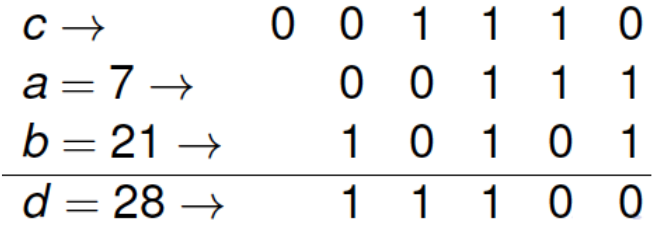
\includegraphics[width = 0.3\textwidth]{img/img30.png}
    \end{center} \vspace{3.5pt}
    The third digits of the numbers $a$ and $b$ are both equal to $1$, therefore, after the sum, we carry the additional digit to the fourth column. \vspace{7pt}

    Through these decision variables, we get four different relationships. Assuming the following equivalance:
    $$ a + b + c = d $$
    the relationships between these boolean variables are divided into:
    \begin{enumerate}
        \item $0 + 0 + 0 = 0$, we carry on $c = 0$
        \item $0 + 0 + 1 = 1$, we carry on $c = 0$
        \item $0 + 1 + 1 = 1$, we carry on $c = 1$
        \item $1 + 1 + 1 = 1$, we carry on $c = 1$
    \end{enumerate}
    The entire system of equivalances described previously must be taken in account and translated in a specific constraint. \vspace{7pt}

    \textbf{Constraints}.
    \begin{itemize}
        \renewcommand{\labelitemi}{-}
        \item Compute $d_i$ from the right to left starting from $c_0 = 0$ \vspace{3.5pt} \\
        The constraint itself is defined by other three subprocesses, like:
        \begin{enumerate}
            \item \textbf{Compute the result digit by digit}. $$ d_i = a_i + b_i + c_i \text{ mod } 2, \text{ for } i = 0, \dots, n - 1 $$
            \item \textbf{Compute the digit of the carry boolean decision variable}. $$ c_{i + 1} = 1 \leftrightarrow a_i + b_i + c_i > 1, \text{ for } i = 0, \dots, n-1 $$
            \item \textbf{Set the final and the initial digits of the carry boolean decision variable to $0$}. $$ c_n = 0 \text{ and } c_0 = 0 $$
        \end{enumerate} \vspace{7pt}

        As we already said, the SAT solver works only with propositional formulas. Therefore, we need to convert these subprocesses into their propositional
        counterparts. They becomes:
        \begin{enumerate}
            \item $$ a_i \leftrightarrow b_i \leftrightarrow c_i \leftrightarrow d_i $$
            \item $$ c_{i+1} \leftrightarrow (a_i \wedge b_i) \vee (a_i \wedge c_i) \vee (b_i \wedge c_i) $$
            \item $$ \neg c_n \wedge \neg c_0 $$
        \end{enumerate}
    \end{itemize}

    Let $f$ be the conjuction of all these formulas. To compute the sum $a + b = d$, the final propositional formula is:
    $$ f \wedge \bigwedge_{i=0}^{n-1} [\neg] a_i \wedge \bigwedge_{i=0}^{n-1} b_i $$
    where:
    \begin{itemize}
        \renewcommand{\labelitemi}{-}
        \item $f \rightarrow$ conjuction of all the previous propositional formula
        \item $\bigwedge_{i=0}^{n-1} [\neg] a_i \rightarrow$ expression of the first number in base $2$
        \item $\bigwedge_{i=0}^{n-1} [\neg] b_i \rightarrow$ expression of the second number in base $2$
    \end{itemize} \vspace{7pt}

    For instance, when $a = 13$ and $b = 7$, we have:
    $$ f \wedge \underbrace{\neg a_1 \wedge a_2 \wedge a_3 \wedge \neg a_4 \wedge a_5}_{a = 13 = 01101} \wedge \underbrace{\neg b_1 \wedge \neg b_2 \wedge b_3 \wedge b_4 \wedge b_5}_{b = 7 = 00111} $$
    for which a SAT solver would return us:
    $$ \underbrace{d_1 \wedge \neg d_2 \wedge d_3 \wedge \neg d_4 \wedge \neg d_5}_{d = 20 = 10100} $$

    If $d$ does not fit in $n$ digits, $c_n$ will be forced to be $1$, and the result will be UNSAT. A quick solution would be to expand the formula with 
    leading bits in $a$ and $b$ set to $0$.
\end{example}